
\documentclass{sig-alternate-05-2015}

\usepackage{hyperref}

\begin{document}

% --- Author Metadata here ---
% Copyright
\setcopyright{rightsretained}

% DOIs
\doi{10.13140/RG.2.1.5130.0882}

% ISBN
%\isbn{123-4567-24-567/08/06}

%Conference
\conferenceinfo{Supercomputing `15: ESnet SDN Workshop}{November 20, Austin, TX}

\CopyrightYear{2015} % Allows default copyright year (20XX) to be over-ridden - IF NEED BE.
%\crdata{0-12345-67-8/90/01}  % Allows default copyright data (0-89791-88-6/97/05) to be over-ridden - IF NEED BE.
% --- End of Author Metadata ---

\title{Data Transfer in a Science DMZ using SDN with Applications for Precision Medicine in Cloud and High-performance Computing}

\numberofauthors{9} %  in this sample file, there are a *total*
% of EIGHT authors. SIX appear on the 'first-page' (for formatting
% reasons) and the remaining two appear in the \additionalauthors section.
% UPDATE: this was changed to be 9 from the original 6 including in the CLS file.

\author{
% You can go ahead and credit any number of authors here,
% e.g. one 'row of three' or two rows (consisting of one row of three
% and a second row of one, two or three).
%
% The command \alignauthor (no curly braces needed) should
% precede each author name, affiliation/snail-mail address and
% e-mail address. Additionally, tag each line of
% affiliation/address with \affaddr, and tag the
% e-mail address with \email.
%
% 1st. author
\alignauthor
Nam Pho\titlenote{The author can be reached at: \href{mailto:nam_pho@hms.harvard.edu}{nam\_pho@hms.harvard.edu}}\\
       \affaddr{Harvard Medical School}\\
       \affaddr{Research Computing}\\
       \affaddr{Boston, USA}\\
%       \email{nam\_pho@hms.harvard.edu}
% 2nd. author
\alignauthor
Dino R. C. Magri\\
       \affaddr{University of S\~{a}o Paulo}\\
       \affaddr{LARC - PCS - EPUSP}\\
       \affaddr{S\~{a}o Paulo, Brazil}\\
%       \email{dino@larc.usp.br}
% 3rd. author
\alignauthor 
Fernando F. Redigolo\\
       \affaddr{University of S\~{a}o Paulo}\\
       \affaddr{LARC - PCS - EPUSP}\\
       \affaddr{S\~{a}o Paulo, Brazil}\\
%       \email{fernando@larc.usp.br}
\and  % use '\and' if you need 'another row' of author names
% 4th. author
\alignauthor Byoung-Do Kim\\
       \affaddr{University of Virginia}\\
       \affaddr{Research Computing}\\
       \affaddr{Charlottesville, USA}\\
%       \email{bdkim@virginia.edu}
% 5th. author
\alignauthor Timothy Feeney\\
       \affaddr{Tufts Medical Center}\\
       \affaddr{Department of Surgery}\\
       \affaddr{Boston, USA}\\
%       \email{tfeeney@tuftsmedicalcenter.org}
% 6th. author
\alignauthor Heidi L. Morgan\\
       \affaddr{Florida International University}\\
       \affaddr{CIARA}\\
       \affaddr{Miami, USA}\\
%       \email{heidi@fiu.edu}
\and
% 7th. author
\alignauthor Chirag J. Patel\\
       \affaddr{Harvard Medical School}\\
       \affaddr{Department of Biomedical Informatics}\\
       \affaddr{Boston, USA}\\
%       \email{chirag@hms.harvard.edu}
% 8th. author
\alignauthor Chris Botka\\
       \affaddr{Harvard Medical School}\\
       \affaddr{Research Computing}\\
       \affaddr{Boston, USA}\\
%       \email{botka@hms.harvard.edu}
% 9th. author
\alignauthor Tereza Cristina M. B. Carvalho\\
       \affaddr{University of S\~{a}o Paulo}\\
       \affaddr{LARC - PCS - EPUSP}\\
       \affaddr{S\~{a}o Paulo, Brazil}\\
%       \email{carvalho@larc.usp.br}
}

% There's nothing stopping you putting the seventh, eighth, etc.
% author on the opening page (as the 'third row') but we ask,
% for aesthetic reasons that you place these 'additional authors'
% in the \additional authors block, viz.
%\additionalauthors{N/A}
%\date{30 July 1999}
% Just remember to make sure that the TOTAL number of authors
% is the number that will appear on the first page PLUS the
% number that will appear in the \additionalauthors section.

\maketitle

\begin{abstract}
As the difficulty and cost of generating data has decreased, there have
been emerging problems of data movement between where it was collected
to where it can most effectively be processed. The Science DMZ model is an
established solution to help maximize the throughput from
any given network infrastructure between sites but there still exists
room for exploration and improvement, including the use of
Software-Defined Networking (SDN). We aim to explore how the use of
SDN-enabled flows in a Science DMZ may impact its main trait:
performance. In this paper we have successfully demonstrated
improvements in data transfer between certain sites and under certain
conditions. Though we have also seen sites where there is no difference
or even a performance penalty, all the results are consistent and
reproducible over hundreds of test transfers suggesting there are unique
properties of each site configuration leading to real and sustained
performance increases to a Science DMZ.

\end{abstract}

\terms{Measurement, Performance, Design, Reliability, Experimentation, Security}

\keywords{Science DMZ; SDN, Software Defined Networking; Brocade; OF, OpenFlow; Genomics; Precision Medicine; Personalized Medicine; Cloud Computing; Top500; HPC, High-performance Computing
}

\section{Introduction}

In early 2015, a little over a decade after the first draft of the human genome was published in 2003, the United States announced a new \$215-million precision medicine initiative \cite{TheWhiteHouse}. Though daunting in scale at its goal to collect high-throughput biological (e.g., genomic) data from millions of individuals, it follows as a natural progression of increasingly larger-scale sequencing studies such as the 1,000 genomes \cite{Altshuler2010}, The Cancer Genome Atlas (TCGA) among others. The exponentially decreasing cost of sequencing an individual's genome has dwarfed the rate of Moore's law and turned medicine into a big data discipline. There are even predictions in the scientific community that it will exceed the storage growth rate of established big data fields such as online video (YouTube), social media (Twitter), and astronomy (Australian Square Kilometre Array Pathfinder project). Conservative estimates put genomics on par with these other fields at two exabytes of genomic data by 2025 to more extreme predictions of up to 20 orders of magnitude more \cite{Stephens2015}. The computational resources required to process this data will also grow in tandem. The second sizable challenge is security. Precision medicine is defined as human-subjects research and must comply to regulation that ensure the privacy and confidentiality of research subjects (e.g., HIPAA). Therefore, the transfer of data must also be secure.

Regardless of the discipline, moving large volumes of data between sites has been increasingly stressed by the ease of data accumulation; pockets of data rich and data poor sites naturally form. Particularly in the genomics field, there is a tension between data production centers, such as those producing next-generation genomic sequencing information, and supercomputing or cloud data centers that have computational resources required to process and analyze data. Through domestic initiatives such as ESnet and Internet2 and international ones between North and South America such as AmLight \cite{Ibarra2015}, improved bandwidth interconnectivity and other data transfer methods were introduced to address increasing data sizes. However, even with sufficient 10 Gigabit bandwidth infrastructure between locales, there are blocks to the natural flow of data such as stateful firewalls that the Science DMZ was created to address \cite{Dart2013}. The concept of a Science DMZ has also been adopted internationally, particularly in Brasil, with a similar nation-wide initiative from Brazil's National Research and Educational Network (RNP - Rede Nacional de Ensino e Pesquisa) led by the University of S\~{a}o Paulo (USP) researchers \cite{Magri2014}.

\section{SDN-enabled Science DMZ}

Software-Defined Networking (SDN) has been a maturing technology that has seen measured rates of adoption in the real-world \cite{Kreutz2014}. The use of a SDN-enabled Science DMZ was proposed by Dart, et al. in 2013 but we describe the implementation and benchmarking of it in practice for genomics. 

At USP we are using a Brocade hybrid Openflow switch (CES-2024C-4X) with the latest firmware update (v5.8.0) for the Science DMZ. The University's border router and the SDN controller are connected to a non-OpenFlow vlan (vlan1), whereas the Data Transfer Node (DTN) has ports both in vlan1 and in an OpenFlow-enabled network segment (vlan4000). A physical loop connects both segments. 

\begin{figure}
\centering
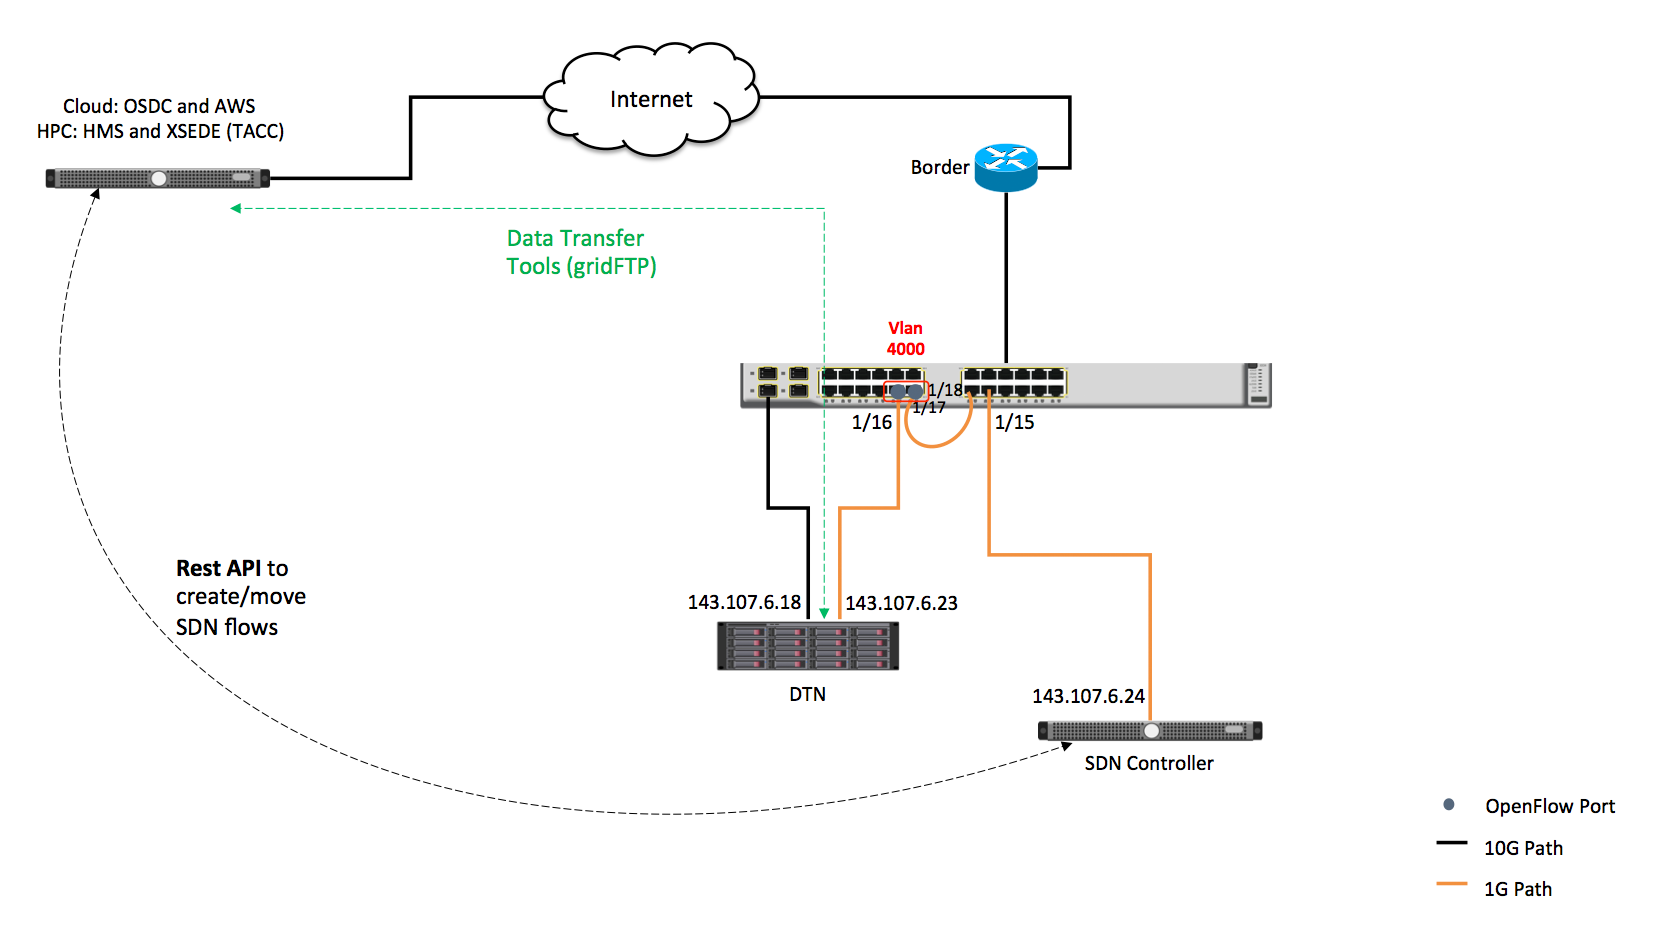
\includegraphics[scale=0.15]{images/arch.png}
\caption{A network diagram of data as it transits the internet from the DTC to the DTN through a Science DMZ}
\label{fig:arch}
\end{figure}

As shown in Figure \ref{fig:arch}, Data Transfer Clients (DTCs) running on different external sites initiate a request for file transfer to the DTN at USP via a REST API call to the SDN controller, which will then insert OpenFlow rules into the switch in order to enable traffic from each DTC to reach the DTN. Upon completion of transfer the flows will subsequently be removed. 

Using the ovs-ofctl OpenFlow command we create four distinct flows on the switch via a REST API on the SDN controller when the request is initiated. Two of them handle ARP packets to and from the DTN. The third directs IP packets destined for the DTN to the OpenFlow-enabled port through the physical internal cable loop, while the last one handles packets leaving the DTN in the reverse direction through the internally looped port bridge. When a transfer is finished another call to the REST API on the SDN controller will destroy the OpenFlow table and prevent packets from reaching the DTN.

\section{Data transfer}

As the goal of any Science DMZ is to optimize data transfers, we aim to show that the use of additional features provided by SDN come at no expense to existing performance. We use one of the first available full genome sequences from an individual as our transfer data set \cite{Levy2007} where the goal is to process and map the genome from raw data at a compute-rich cloud or HPC site then transfer the assembled sequence via USP's Science DMZ. All machines involved are running Linux (CentOS 6.6) using GridFTP 5.2.5 for the transfer agent. As disk latency is known to also be a factor in data transfer we will try different storage options on the DTC to a local RAID-1 disk on the DTN at the Science DMZ. In each condition we will perform 100 file transfers and record their average speed in Mbps.

\subsection{Personalized Medicine}

The chemical DNA of an individual is comprised of approximately 2.8 billion base pairs (bps) divided into 23 pairs of chromosomes of which each base is represented by a single IUPAC code as ASCII on disk with accompanying metadata. The most common method of sequencing a genome involves shearing chemical DNA into fragments of several hundred bps and sequencing each fragment from one or both ends, using the sequence piece to map to a reference genome. The mapping process is computationally intensive though embarrassingly parallel in nature. The genome to be assembled and transferred was sequenced at 7.5-fold coverage and is 180 Gb of raw data and 2.8 Gb of processed data on disk though the standard now is commonly 30-fold coverage or greater. Details on the raw data and processing protocol are beyond the scope of this paper and can be described in detail in Levy, et al.

\subsection{Academic and Commercial Clouds}

Cloud computing is an attractive option for processing data as it allows for elasticity; the cloud can dynamically scale to fit the task at hand and costs are only commensurate with the resources required of a project. Despite the availability of cloud solutions, adoption of it has been slow for research projects though in recent years regulatory and funding support has caught up to the changing research paradigm \cite{Stein2015}. 

The Open Science Data Cloud (OSDC) is an academic cloud and data commons running OpenStack hosted at the University of Chicago \cite{Stein2015}. Academic clouds are useful for being specialized to individual research domains and more forgiving as a private research environment. For example, Bionimbus is an academic cloud for biomedical research providing a central data commons in conjunction with the elastic compute services \cite{Heath2014}. In our example we are running a m1.large instance on the OSDC with virtual and GlusterFS storage options as a DTC.

In the commercial cloud computing space players such as Google, Amazon, Microsoft, and Rackspace have established solutions. The benefit of a commercial solution is the proprietary engineering behind each cloud, which is often derived from the company's experience delivering other services through their proven global infrastructure. Using the Amazon Web Services (AWS) cloud a DTC was provisioned on an m3.xlarge instance with a SSD backed EBS in the Northern Virginia (US) zone. 

\begin{figure}
\centering
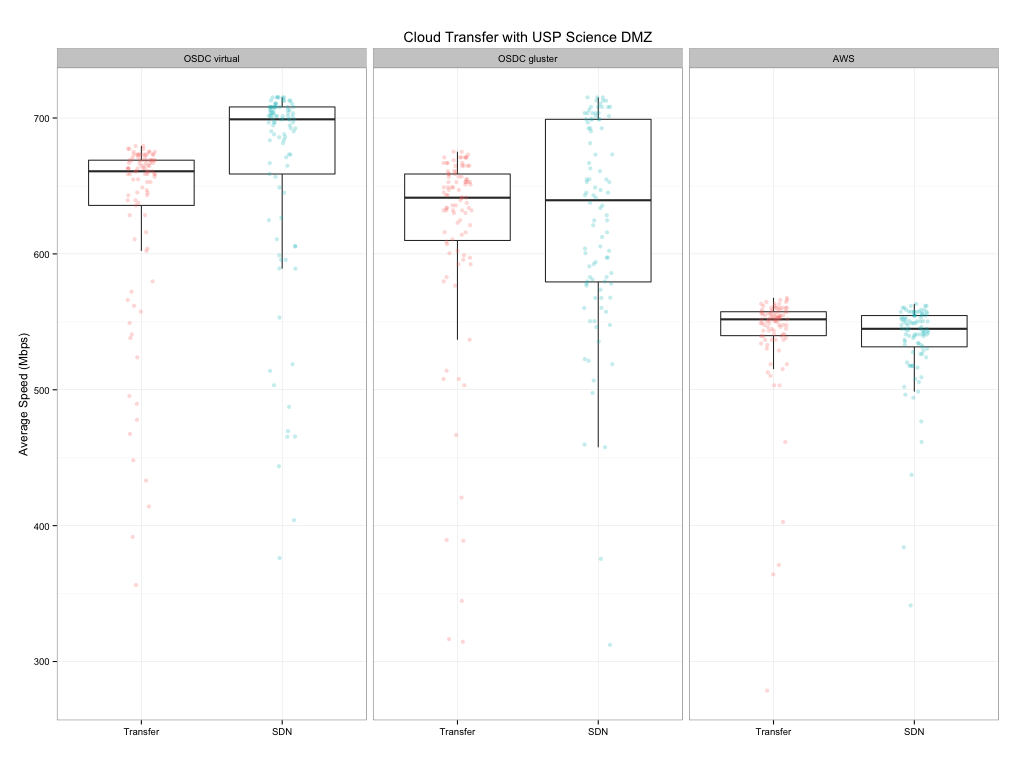
\includegraphics[scale=0.23]{images/cloud.png}
\caption{Genome transfer using GridFTP with and without OpenFlow enabled between academic (OSDC) and commercial (AWS) clouds with the USP Science DMZ}
\label{fig:cloud}
\end{figure}

When transferring from a virtual filesystem on OSDC we experienced statistically significantly faster data transfers (p=2.45e-3), an increase from 630 to 663 Mbps on average at 5\% improved throughput (Figure \ref{fig:cloud}, left panel). Using the same DTC on OSDC with the GlusterFS volume we experienced no change in data transfer performance (p=0.379) from the normal transfer at 615 Mbps on average though the variability in speeds increased 2.4-fold from an IQR of 48.9 to 120 Mbps under SDN transfers (Figure \ref{fig:cloud}, middle panel).

Using AWS we saw slower average file transfer speeds compared to the OSDC and no difference in speed using normal or SDN-enabled flows (p=0.538). However, there was much greater consistency for each transfer at 539 Mbps on average for normal conditions and only a 5.44 Mbps difference in IQR between normal and SDN flows in AWS (Figure \ref{fig:cloud}, right panel).

\subsection{Top500 and Academic Medical HPC Centers}

Supercomputing sites such as those found in the Top500 are an attractive solution to help process data; a network of HPC centers form the backbone of the Extreme Science and Engineering Discovery Environment (XSEDE) consortium in the US \cite{Towns2014}. Among one of the sites is the Stampede supercomputer at the Texas Advanced Computing Center (TACC), among the top 10 clusters in the world as measured by more than 5,000 Teraflops of processing power. At TACC the data was staged for file transfer on two separate production Lustre-based storage devices functioning as home and scratch directories. 

In the area of precision medicine, genomes are processed locally to where the samples are collected at academic medical centers and supporting HPC facilities are the first to analyze the data. For example, the Orchestra cluster has over 7,000 CPU cores to support Harvard Medical School (HMS) and its 12 affiliated hospitals in all fields of biomedical research. At HMS the transfer data was staged on a local SSD storage volume.

\begin{figure}
\centering
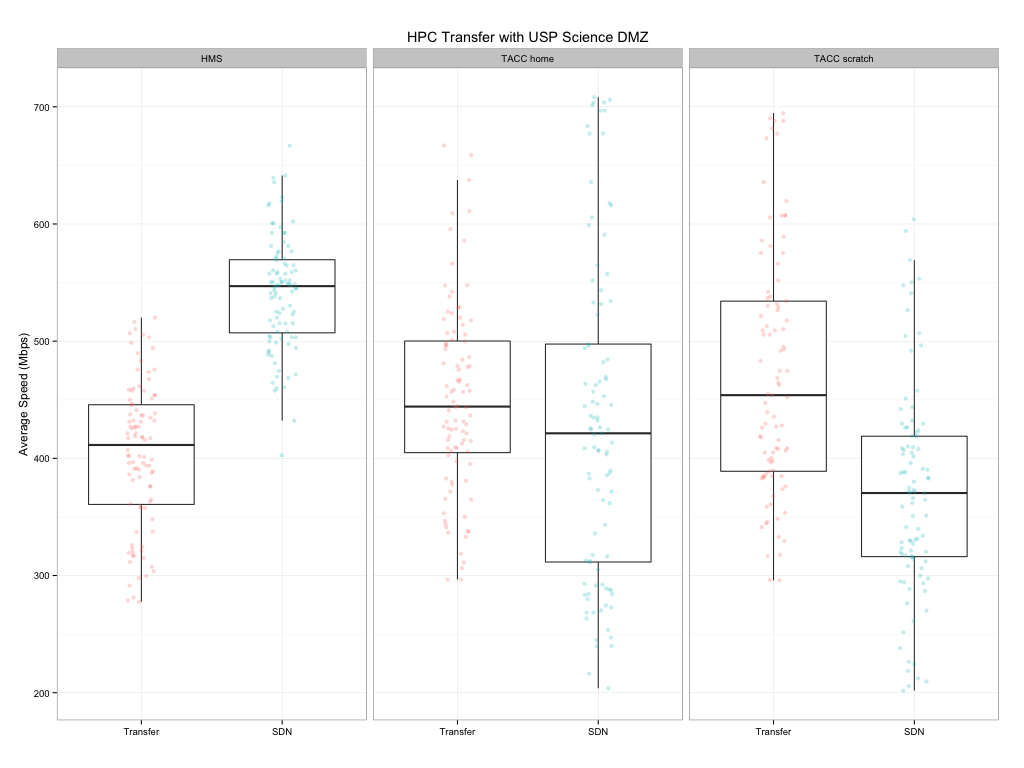
\includegraphics[scale=0.23]{images/hpc.png}
\caption{Genome transfer using GridFTP with and without OpenFlow enabled between Top500 (TACC) and academic medical (HMS) supercomputing centers with the USP Science DMZ.}
\label{fig:hpc}
\end{figure}

Using the DTC at HMS we demonstrated a statistically significant increase in file transfer performance using SDN (p = 2.2e-16). Speeds to USP increased from 403.2 Mbps (sd=61.6) to 541.0 Mbps (sd=48.2) on average, a 34.2\% increase in performance throughput  (Figure \ref{fig:hpc}, left panel). 

From the TACC site there were mixed results with no change in average file transfer performance speeds using home (p = 0.199) but a performance penalty under scratch (p=3.55e-11) designated Lustre devices. Using the home device we averaged 450.3 Mbps of transfer while under scratch the average speed decreased from 470.8 to 371.0 Mbps, a performance degradation of 21\% (Figure \ref{fig:hpc}, middle and right panels).

\section{Discussion}

Though Science DMZs have been an established technology to improve data transfer performance, we sought to explore methods of further optimizing it or extending its functionality by means of the SDN paradigm. Through our exploratory survey we received mixed results including performance increases at the OSDC (virtual) and HMS, indifferent results through AWS and OSDC (GlusterFS) and TACC (home), and even performance decreases at TACC (scratch). Given that each of these transfer sites is a production environment and tests were done over multiple days it is difficult to control with 100\% certainty all potential confounding variables. For example, internal TACC benchmarks have the scratch device capable of 160 GBps of max throughput versus 12 GBps for home. Neither of these should be rate limiting properties for our tests yet file transfers from TACC using scratch had worse performance under SDN flows.

SDN-enabled Science DMZs remain a viable option for optimizing the secure transfer of potentially private genomics data on many thousands of individuals, however we have shown that performance is context dependent and confounded. The results presented are promising and we recommend further study and consideration. In particular, it is our intent to execute increased testing under more controlled conditions to better understand enabling and penalizing factors for SDN-enabled data transfer. Future work includes extending the protocol between the DTC and SDN controllers for supporting additional features, such as improved security methods through key-based authentication prior to flow modification and using dynamically provisioned Layer-2 circuits (such as the ones provided by Internet2 ION service) for lower latency data transfers to the DTN.   

\section{Acknowledgments}
N.P. was supported in part by the National Science Foundation grant number 1129076 for PIRE: Training and Workshops in Data Intensive Computing Using The Open Science Data Cloud.

We would like to acknowledge the National Science Foundation grant number 1129076 for funding the Center for Data Intensive Science at the University of Chicago and the Center for Internet Augmented Research and Assessment (CIARA) at Florida International University.

Portions of this research were conducted on the Orchestra High Performance Compute Cluster at Harvard Medical School. This NIH supported shared facility consists of thousands of processing cores and terabytes of associated storage and is partially provided through grant NCRR 1S10RR028832-01.

This work also used the Extreme Science and Engineering Discovery Environment (XSEDE), which is supported by National Science Foundation grant number ACI-1053575.

This research was also supported by RNP Science DMZ program. We also would like to acknowledge USP DTI (Information Technology Department from USP) for the support. 

\bibliographystyle{abbrv}
\bibliography{refs}

\end{document}
